\documentclass[12pt]{article}
\usepackage{amsmath}
\usepackage{graphicx}
\usepackage{float}
\usepackage{mathtools}
\usepackage{tikz}
\usepackage{pgfplots}
\begin{document}
\title{Computer Science 145, Homework 2}
\date{February 5th, 2019}
\author{Michael Wu\\UID: 404751542}
\maketitle

\section*{Problem 1}

\paragraph{a)}

There are 10 democrats and 10 republicans. This has an entropy of 1.
If we first split the data set by the vote for handicapped infants,
the no category will have 4 democrats and 8 republicans. The yes
category will have 6 democrats and 2 republicans. The entropy is
given by the following expression.
\begin{multline*}
    \frac{3}{5}\left(-\frac{1}{3}\log_2\left(\frac{1}{3}\right)-\frac{2}{3}\log_2\left(\frac{2}{3}\right)\right)\\
    +\frac{2}{5}\left(-\frac{1}{4}\log_2\left(\frac{1}{4}\right)-\frac{3}{4}\log_2\left(\frac{3}{4}\right)\right)\approx 0.87549
\end{multline*}

If we first split the data set by the vote for water project cost
sharing, the no category will have 6 democrats and 4 republicans.
The yes category will have 4 democrats and 6 republicans. Since
the entropy is the same for both the yes and the no categories,
it is given by the following expression.
\[-\frac{3}{5}\log_2\left(\frac{3}{5}\right)-\frac{2}{5}\log_2\left(\frac{2}{5}\right)\approx 0.97095\]

If we first split the data set by the vote for budget resolution
adoption, the no category will have 1 democrat and 8 republicans.
The yes category will have 9 democrats and 2 republicans.
The entropy is given by the following expression.
\begin{multline*}
    \frac{9}{20}\left(-\frac{1}{9}\log_2\left(\frac{1}{9}\right)-\frac{8}{9}\log_2\left(\frac{8}{9}\right)\right)\\
    +\frac{11}{20}\left(-\frac{2}{11}\log_2\left(\frac{2}{11}\right)-\frac{9}{11}\log_2\left(\frac{9}{11}\right)\right)\approx 0.60269
\end{multline*}
Clearly we should first split the data by the vote for budget resolution adoption,
since it has an information gain of \(1-0.60269=0.39731\) which is higher than any of the other options.

Let's look at the no branch. It starts with an entropy of
\[-\frac{1}{9}\log_2\left(\frac{1}{9}\right)-\frac{8}{9}\log_2\left(\frac{8}{9}\right)\approx0.50326\]
and if we split by the vote for handicapped infants the no branch will have 1 democrat and 7 republicans. The yes
branch will have 1 republican. The yes branch has 0 entropy, so the entropy after the split is the following.
\[\frac{8}{9}\left(-\frac{1}{8}\log_2\left(\frac{1}{8}\right)-\frac{7}{8}\log_2\left(\frac{7}{8}\right)\right)\approx 0.48317\]

If we split the no branch by the vote for water project cost sharing, the no branch will have 3 republicans and the yes branch
will have 1 democrat and 5 republicans. Then the entropy is the following.
\[\frac{2}{3}\left(-\frac{1}{6}\log_2\left(\frac{1}{6}\right)-\frac{5}{6}\log_2\left(\frac{5}{6}\right)\right)\approx 0.43335\]
Then we should split by the vote for water project cost sharing since it has the higher information gain of \(0.50326-0.43335=0.06991\).
This only leaves one feature to split by, resulting in a prediction of republican for every option on the no branch of the first node.

On the yes branch of the first node, we start with an entropy of
\[-\frac{2}{11}\log_2\left(\frac{2}{11}\right)-\frac{9}{11}\log_2\left(\frac{9}{11}\right)\approx0.68404\]
and if we split by the vote for handicapped infants the no branch will have 3 democrats and 1 republican. The yes branch will have
6 democrats and 1 republican. If we split by the vote for water project cost sharing, then the no branch will have 6 democrats
and 1 republican, while the yes branch will have 3 democrats and 1 republican. So either selection will lead to the same split
and result in the same entropy. This is given by the following.
\begin{multline*}
    \frac{4}{11}\left(-\frac{1}{4}\log_2\left(\frac{1}{4}\right)-\frac{3}{4}\log_2\left(\frac{3}{4}\right)\right)\\
    +\frac{7}{11}\left(-\frac{1}{7}\log_2\left(\frac{1}{7}\right)-\frac{6}{7}\log_2\left(\frac{6}{7}\right)\right)\approx 0.67153
\end{multline*}
The information gain is \(0.68404-0.67153=0.01251\). In this case I will choose to split by the vote for handicapped infants.
Then the next split will be the vote for water project cost sharing. There is one path that leads to a 50/50 split if there is a
no vote for handicapped infants, a yes vote for water project cost sharing, and a yes vote for budget resolution adoption. The remainder
of the options on the yes side of the first node should be democrat. Then the tree will look like the following.
\begin{figure}[H]
    \begin{center}
        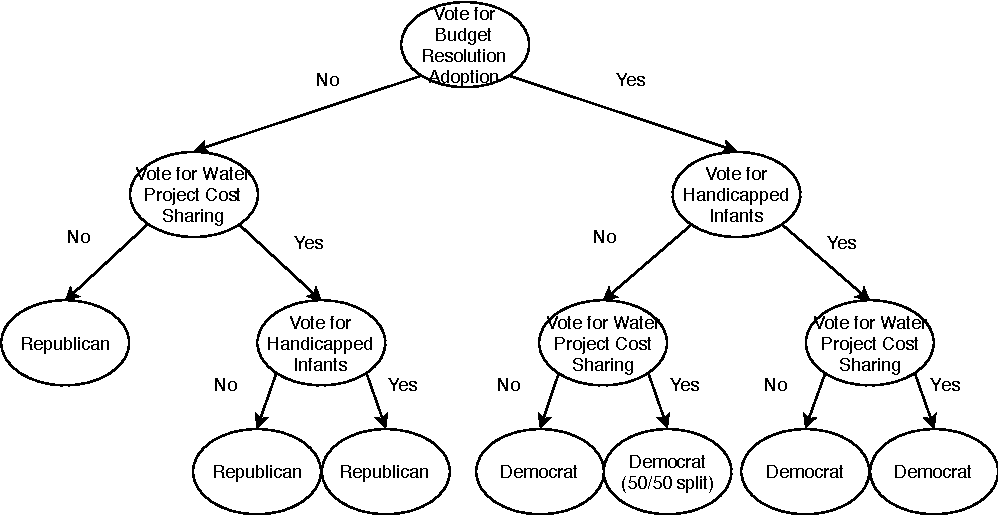
\includegraphics[width=5in]{DecisionTree.pdf}
    \end{center}
\end{figure}
\pagebreak
Because the left and right sides of the first node all have the same end result, this decision tree could be simplified to the following.
\begin{figure}[H]
    \begin{center}
        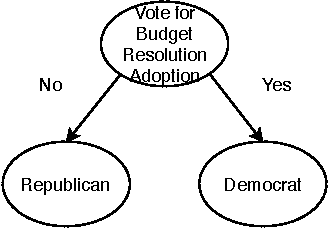
\includegraphics[width=2in]{DecisionTreeSimplified.pdf}
    \end{center}
\end{figure}

\paragraph{b)}

Running the information gain algorithm yields the following decision tree and accuracy.
\scriptsize
\begin{verbatim}
{'legs': {0: {'fins': {0.0: {'toothed': {0.0: 7.0, 1.0: 3.0}},
                       1.0: {'eggs': {0.0: 1.0, 1.0: 4.0}}}},
          2: {'hair': {0.0: 2.0, 1.0: 1.0}},
          4: {'hair': {0.0: {'toothed': {0.0: 7.0, 1.0: 5.0}}, 1.0: 1.0}},
          6: {'aquatic': {0.0: 6.0, 1.0: 7.0}},
          8: 7.0}}
Test accuracy:  0.8571428571428571
\end{verbatim}
\normalsize
Running the gain ration algorithm yields the following decision tree and accuracy.
\scriptsize
\begin{verbatim}
{'feathers': {0: {'backbone': {0.0: {'airborne': {0.0: {'predator': {0.0: 6.0,
                                                                     1.0: 7.0}},
                                                  1.0: 6.0}},
                               1.0: {'milk': {0.0: {'fins': {0.0: {'legs': {0.0: 3.0,
                                                                            4.0: 5.0}},
                                                             1.0: 4.0}},
                                              1.0: 1.0}}}},
              1: 2.0}}
Test accuracy:  0.8095238095238095
\end{verbatim}
\normalsize
I would choose the information gain algorithm, as it leads to higher accuracy. The gain
ratio algorithm unfairly punishes using legs as a selection feature, even though legs
is a very good characteristic when trying to distinguish between animal types.

\section*{Problem 2}

\paragraph{a)}

The support vectors are points 2, 6, and 18 which are given by the tuples shown below.
\[(0.91, 0.32, 1)\qquad (0.41, 2.04, 1)\qquad(2.05, 1.54, -1)\]

\paragraph{b)}

The normal vector can be calculated as shown below.
\[w=0.5084\begin{bmatrix}
    0.91\\
    0.32
\end{bmatrix}+0.4635\begin{bmatrix}
    0.41\\
    2.04
\end{bmatrix}-0.9709\begin{bmatrix}
    2.05\\
    1.54
\end{bmatrix}=\begin{bmatrix}
    -1.337666\\
    -0.386958
\end{bmatrix}\]

\paragraph{c)}

This can be calculated as follows.
\[b=\frac{\splitfrac{1-0.91*(-1.337666)-0.32*(-0.386958)}{\splitfrac{+1-0.41*(-1.337666)-2.04*(-0.386958)}{-1-2.05*(-1.337666)-1.54*(-0.386958)}}}{3}=2.33902354\]

\paragraph{d)}

\[f(x)=-1.337666x_1-0.386958x_2+2.33902354\]

\paragraph{e)}

The decision function would output a value of
\[-1.337666-0.386958+2.33902354=0.61439954\]
which is positive, so the predicted class label would be 1. Note that this point is closer to the decision boundary than any of the support vectors.

\paragraph{f)}

The following plot show the data and the decision boundary. The red circles are positive data points and the blue x's are negative data points.
\begin{center}
    \begin{tikzpicture}
        \begin{axis}[scatter/classes={p={mark=o,draw=red},n={mark=x,draw=blue}}, xlabel={\(x_1\)}, ylabel={\(x_2\)}]
            \addplot[scatter,only marks, scatter src=explicit symbolic]
            table[meta=label] {
                x y label
                0.52 -1 p
                0.91 0.32 p
                -1.48 1.23 p
                0.01 1.44 p
                -0.46 -0.37 p
                0.41 2.04 p
                0.53 0.77 p
                -1.21 -1.1 p
                -0.39 0.96 p
                -0.96 0.08 p
                2.46 2.59 n
                3.05 2.87 n
                2.2 3.04 n
                1.89 2.64 n
                4.51 -0.52 n
                3.06 1.3 n
                3.16 -0.56 n
                2.05 1.54 n
                2.34 0.72 n
                2.94 0.13 n
            };
            \addplot[thick, draw=black, mark=none, domain={1:2}] {6.04464 - 3.45688*x};
        \end{axis}
    \end{tikzpicture}
\end{center}

\end{document}